Nachvollziehbarkeit bedeutet allgemein, dass über ein resultierendes Verhalten eines Systems auch interne Zustände nachvollzogen werden können. Dies ist keine neue Idee, sondern fand bereits 1960 im Gebiet der Kontrolltheorie starke Bedeutung \cite{OnTheGeneralTheoryOfControlSystems}. Nach Freedman \cite{TestabilityOfSoftwareComponents} und Scrocca \etal \cite{EnablingEventDrivenObservability} lässt sich diese Definition auch auf Softwaresysteme übertragen.
	
In dieser Arbeit wird sich mit der Nachvollziehbarkeit in speziellen Situation befasst, nämlich wenn die Stakeholder das Verhalten einer Webapplikation und die Interaktionen eines Nutzers verstehen möchten.% Dies bedeutet auch, dass keine allgemeine Nachvollziehbarkeit das Ziel ist, denn z.B. das Nutzer die internen Zustände eines Systems nachvollziehen können, ist nicht das Ziel.
	
\subsection{Nutzen}
	
Tritt beispielsweise ein Softwarefehler (Bug) bei einem Nutzer auf, aber die Stakeholder erhalten nicht ausreichende Informationen, so kann der Bug ignoriert werden oder gering priorisiert und in Vergessenheit geraten. Dies geschah im Jahr 2013, als Khalil Shreateh eine Sicherheitslücke bei Facebook fand und diesen bei Facebooks Bug-Bounty-Projekt Whitehat meldete \cite{FacebookBugBounyHunt}. Sein Fehlerreport wurde aufgrund mangelnder Informationen abgelehnt:
	
\begin{quotation}
Unfortunately your report [...] did not have enough technical information for us to take action  on  it. We  cannot  respond  to  reports  which  do  not contain enough detail to allow us to reproduce an issue.
\end{quotation}
	
Durch den Bug konnte Shreateh auf die private Profilseite von Nutzern schreiben, ohne dass er mit ihnen vernetzt war. Um Aufmerksamkeit auf das Sicherheitsproblem zu erregen, hinterließ er eine Nachricht auf Facebooks Gründer und CEO Mark Zuckerbergs Profilseite. Erst hiernach nahm sich Facebooks Team dem Problem an.
	
\subsection{Nachvollziehbarkeit bei SPAs}
	
Wie zuvor in \autoref{sec:clientbased-webapps} ``\nameref{sec:clientbased-webapps}`` geschildert, gibt es bei Webapplikationen und insbesondere Singe-Page-Applications besondere Barrikaden, die es den Stakeholdern erschwert das Verhalten einer Applikation und die Interaktionen eines Nutzers nachzuvollziehen.
	
Bei SPAs ist die Hauptursache, dass die eigentliche Applikation nur beim Client läuft und nur gelegentlich mit einem Backend kommuniziert.
	
% Im nächsten Kapitel werden Methoden und Konzepte beschrieben, wie man in Softwareprojekten die Nachvollziehbarkeit verbessern kann.

% In dieser Arbeit werden SPAs untersucht, denn einerseits fallen diese in das Interessengebiet der Open Knowledge, anderseits gibt es aber auch einige Eigenheiten, die die Nachvollziehbarkeit reduzieren. Beispielsweise gehen durch die starke Trennung von Client und Server auch Kontextinformationen verloren. Zudem wird die Applikation beim Client größer und komplexer, welches das Potenzial von Ungereimtheiten erhöht.

\subsection{Hürden bei Browsern}

% Zusätzlich zu der Sandbox gibt es weitere Vorkehrungen, die definieren welche Daten innerhalb der JavaScript Umgebung abgerufen und mit welchen Diensten kommuniziert werden darf \cite{LearningJavaScript}. Zwei wichtige dieser Vorkehrungen, die eine Webapplikationen nutzen kann bzw. beachten muss, werden folgend erklärt.

\subsubsection{Cross-Origin Resource Sharing (CORS)}

Wie in der Geschichte zu JavaScript beschrieben, stellt CORS eine natürliche Entwicklung zur Erweiterung des Funktionsumfangs von JavaScript dar. Um nicht auf einen einzelnen Webserver beschränkt zu sein, wurde mit CORS diese Einschränkung eingegrenzt. Wichtiger Bestandteil von CORS ist aber eher die Absicherung vor Missbrauch, weswegen die Einschränkungen überhaupt existierte. Das Konzept von CORS stellt sicher, dass aus einer JavaScript-Umgebung heraus keine Ressourcen von Webservern angefragt werden, außer diese Webserver stimmen der Anfrage zu \cite{MDNCORS}.

In \autoref{fig:cors-workflow} kann betrachtet werden, wie eine ``cross-origin`` Ajax-Anfrage nach dem Konzept von CORS gehandhabt wird. Hierbei ist zu sehen, dass wenn der Aufruf nicht standardmäßig\footnotemark ist, der Browser eine zusätzliche OPTIONS Anfrage an den jeweiligen Webserver sendet - dies stellt einen sogenannten ``Preflighted Request`` dar. Wenn der Webserver in seiner Antwort auf die OPTIONS Anfrage nun bestätigt, dass die Methode, die Header und der ``Content-Type`` so erlaubt sind, wird auch die eigentliche Ajax-Anfrage ausgeführt. Ansonsten schlägt die Anfrage fehl und im JavaScript-Kontext ist lediglich der Fehlschlag zu sehen, ohne einen Hinweis auf die Diskrepanz bzgl. CORS.

\footnotetext{Standardmäßig ist eine Anfrage, wenn 1. die Methode GET, HEAD oder POST entspricht; 2. keine eigene Headern enthält; und 3. der ``Content-Type`` von POST-Anfragen einem der folgenden Werte entspricht: ``application/x-www-form-urlencoded``, ``multipart/form-data`` oder ``text/plain`` \cite{MDNCORS}.}

\begin{figure}[H]
	\centering
	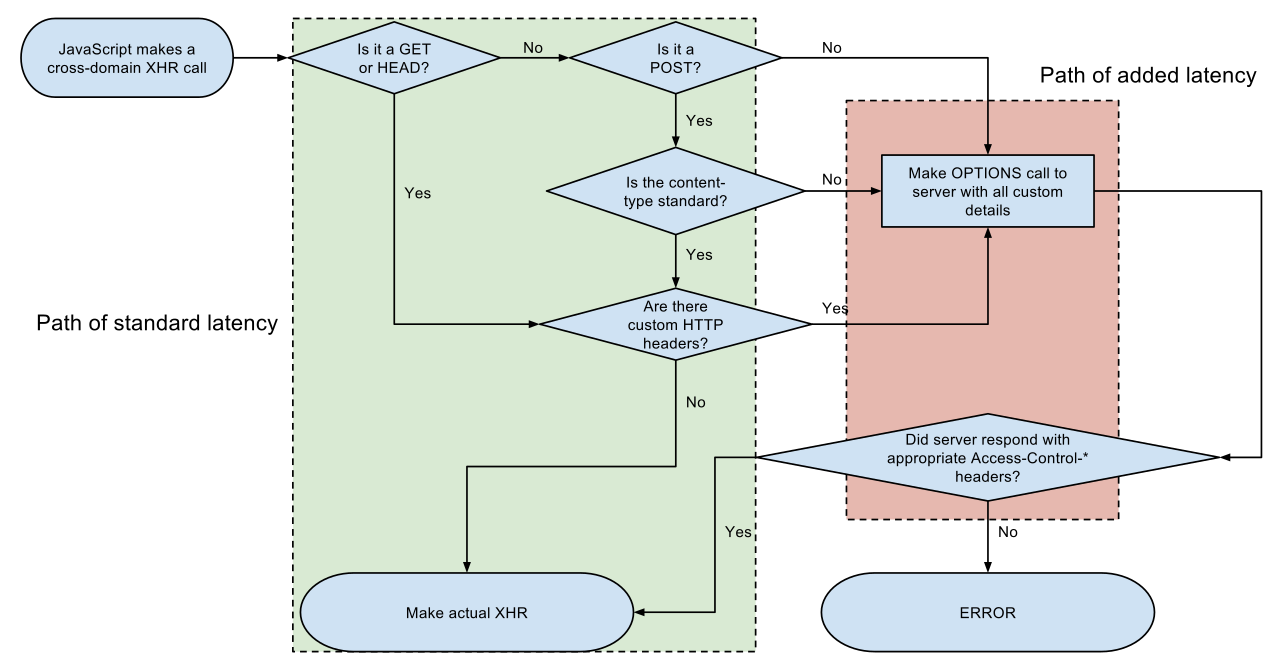
\includegraphics[width=\linewidth]{img/02_theorie/1280px-Flowchart_showing_Simple_and_Preflight_XHR.svg.png}
	\caption{Flowchart über den Ablauf von Ajax-Anfragen mit CORS \cite{FlowchartCORS}}
	\label{fig:cors-workflow}
\end{figure}

%Folgendes vereinfachtes Beispiel soll den Nutzen und den generellen Ablauf von CORS näher erläutern:
%
%\begin{quotation}
%Ein Nutzer ruft eine Webapplikation auf, welche unter \texttt{localhost:3000} bereitgestellt wird. Diese Webapplikation sendet, für den Nutzer unwissend, Anfragen an einen Facebook Dienst. Dies lässt der Browser aber nur zu, wenn der Dienst von Facebook explizit bestätigt, dass eine Anfrage von \texttt{localhost:3000} diese Aktion ausführen darf.
%
%Dafür sendet der Browser eine OPTIONS-Anfrage, in der die Herkunft (``Origin``) der Anfrage notiert ist. Der Facebook Dienst antwortet daraufhin mit den entsprechenden CORS-Headern und gibt somit an, ob die Anfrage von dieser Origin aus erlaubt ist. Nun prüft der Browser, ob die von Facebook übermittelten Origins übereinstimmen. Ist dies nicht der Fall, wird die Anfrage im Browser blockiert und im JavaScript Kontext schlägt dieser fehl. Details zum Fehler werden der JavaScript-Umgebung bewusst enthalten.
%\end{quotation}

\subsubsection{Content-Security-Policy}

\nomenclature[Fachbegriff]{CSP}{Content-Security-Policy}
\nomenclature[Fachbegriff]{XSS}{Cross-Site-Scripting}
\nomenclature[Fachbegriff]{CDN}{Content Delivery Network}

Eine Content-Security-Policy (CSP) definiert, welche Funktionalitäten einer Webapplikation aus geladen zur Verfügung stehen. Dies dient unter anderem dem Schutz vor Cross-Site-Scripting, indem eine Webapplikation beschränken kann, welche Funktionalitäten in JavaScript verfügbar sind und von wo aus JavaScript und CSS Skripte geladen werden dürfen \cite{MDNContentSecurityPolicy}. Weiterhin kann bei einem Versuch der Webapplikation die Regeln zu umgehen Bericht darüber erstattet werden.

%Nachfolgendes Beispiel soll den Nutzen etwas näher bringen:

%\begin{quotation}
%Eine Webapplikation, welche zwei numerische Eingaben von einem Nutzer entgegennimmt und darauf basierend eine komplexe Operation ausführt und das Ergebnis anzeigt. Diese Operation wird über ein eingebundenes Skript von einem CDN bereitgestellt. Weiterhin wird die Datenverarbeitung über ein eigens bereitgestelltes Skript durchgeführt. Da wir unseren Anwendungsfall kennen, kann durch die Härtungsmaßnahme einer CSP die Webapplikation abgesichert werden. Hierfür werden die Funktionalitäten auf das Folgende beschränkt:
%
%\begin{itemize}
%	\item Das Laden von JavaScript vom eigenen Webserver (\textbf{self}) und vom CDN.
%	\item Das Laden von \texttt{inline}-Skripten wird nicht erlaubt (und ist damit verboten).
%	\item Bei Verstoß soll ein Bericht an einen eigenen Protokollserver gesendet werden.
%\end{itemize}
%
%Die entsprechende CSP sieht wie folgt aus:
%
%\begin{verbatim}
%Content-Security-Policy: default-src 'self'; script-src 'self' example.com;
%\end{verbatim}
%
%Wird nun das Skript des CDN kompromittiert und versucht 
%\end{quotation}

\subsection{Logdaten}

Ähnlich wie bei anderen Umgebungen gibt es eine standardisierte Log- bzw. Konsolenausgabe für die JavaScript Umgebung \cite{MDNConsole}. Diese Ausgabe ist aber für den Standard-Benutzer eher unbekannt und der Zugriff darauf sowie die Funktionen dessen können je nach Browser variieren. Deswegen kann in den meisten Fällen nicht darauf gehofft werden, dass die Nutzer dieses Log bereitstellen. Zusätzlich ist es durch die zuvor beschrieben Härtungsmaßnahmen von Browsern nicht möglich das Log in eine Datei zu schreiben.

Eine Automatisierung der Logdatenerhebung ist zudem auch nicht trivial, denn die Daten, welche in die Ausgabe geschrieben werden, sind nicht aus der JavaScript Umgebung aus lesbar. Alternativ können die Daten selber erhoben oder abgefangen werden. Hierbei besteht aber weiterhin die Hürde, wie die Daten an die Stakeholder gelangen.

\subsection{Fernzugriff}

Ein weiterer Punkt, der die Umgebung ``Browser`` von anderen unterscheidet, ist dass die Stakeholder sich normalerweise nicht auf die Systeme der Nutzer schalten können. Bei Expertenanwendungen ginge dies vielleicht, aber wenn eine Webapplikation für den offenen Markt geschaffen ist, sind die Nutzer zahlreich und unbekannt.

Weiterhin gibt es standardmäßig keine Funktionalität wie z. B. das Remote Application Debugging \cite{JavaDebugWireProtocol}, welches Java unterstützt.